\everymath{\displaystyle}
%\documentclass[pdftex,a4paper]{article}
\documentclass[a4paper]{article}
%%classes: article, report, book, proc, amsproc

%%%%%%%%%%%%%%%%%%%%%%%%
%% Misc
% para acertar os acentos
\usepackage[brazilian]{babel} 
%\usepackage[portuguese]{babel} 
% \usepackage[english]{babel}
% \usepackage[T1]{fontenc}
% \usepackage[latin1]{inputenc}
\usepackage[utf8]{inputenc}
\usepackage{indentfirst}
\usepackage{fullpage}
% \usepackage{graphicx} %See PDF section
\usepackage{multicol}
\setlength{\columnseprule}{0.5pt}
\setlength{\columnsep}{20pt}
%%%%%%%%%%%%%%%%%%%%%%%%
%%%%%%%%%%%%%%%%%%%%%%%%
%% PDF support

\usepackage[pdftex]{color,graphicx}
% %% Hyper-refs
\usepackage[pdftex]{hyperref} % for printing
% \usepackage[pdftex,bookmarks,colorlinks]{hyperref} % for screen

%% \newif\ifPDF
%% \ifx\pdfoutput\undefined\PDFfalse
%% \else\ifnum\pdfoutput > 0\PDFtrue
%%      \else\PDFfalse
%%      \fi
%% \fi

%% \ifPDF
%%   \usepackage[T1]{fontenc}
%%   \usepackage{aeguill}
%%   \usepackage[pdftex]{graphicx,color}
%%   \usepackage[pdftex]{hyperref}
%% \else
%%   \usepackage[T1]{fontenc}
%%   \usepackage[dvips]{graphicx}
%%   \usepackage[dvips]{hyperref}
%% \fi

%%%%%%%%%%%%%%%%%%%%%%%%


%%%%%%%%%%%%%%%%%%%%%%%%
%% Math
\usepackage{amsmath,amsfonts,amssymb}
% para usar R de Real do jeito que o povo gosta
\usepackage{amsfonts} % \mathbb
% para usar as letras frescas como L de Espaco das Transf Lineares
% \usepackage{mathrsfs} % \mathscr

% Oferecer seno e tangente em pt, com os comandos usuais.
\providecommand{\sin}{} \renewcommand{\sin}{\hspace{2pt}\mathrm{sen}}
\providecommand{\tan}{} \renewcommand{\tan}{\hspace{2pt}\mathrm{tg}}

% dt of integrals = \ud t
\newcommand{\ud}{\mathrm{\ d}}
%%%%%%%%%%%%%%%%%%%%%%%%



\begin{document}

%%%%%%%%%%%%%%%%%%%%%%%%
%% Título e cabeçalho
%\noindent\parbox[c]{.15\textwidth}{\includegraphics[width=.15\textwidth]{logo}}\hfill
\parbox[c]{.825\textwidth}{\raggedright%
  \sffamily {\LARGE

Cálculo Diferencial e Integral: Notas de Aula

Domínio e Imagem em gráficos, e Noção de limite

\par\bigskip}
{Prof: Felipe Figueiredo\par}
{\url{http://sites.google.com/site/proffelipefigueiredo}\par}
}

Versão: \verb|20160303|

%%%%%%%%%%%%%%%%%%%%%%%%


%%%%%%%%%%%%%%%%%%%%%%%%
\section{Objetivos de aprendizagem}

Ao final desta aula o aluno deve saber \ldots


\section{Pré-requitos da aula}

\begin{itemize}
\item Domínio e imagem
\item Tabela de valores de uma função
\end{itemize}

\section{Conteúdo}

O aluno deve consultar o livro texto na seção 1.7 para se aprofundar
no conteúdo desta aula.

\subsection{Problema}

Como identificar no plano cartesiano o domínio e a imagem do gráfico de uma função?

\subsection{Domínio e Imagem no gráfico}

Começar com alguns gráficos (ainda sem mostrar a expressão de cada função) e perguntar qual é o intervalo que corresponde ao domínio e à imagem de cada função.

\subsubsection{Exemplo 1}

\begin{figure}[h!]
  \centering
  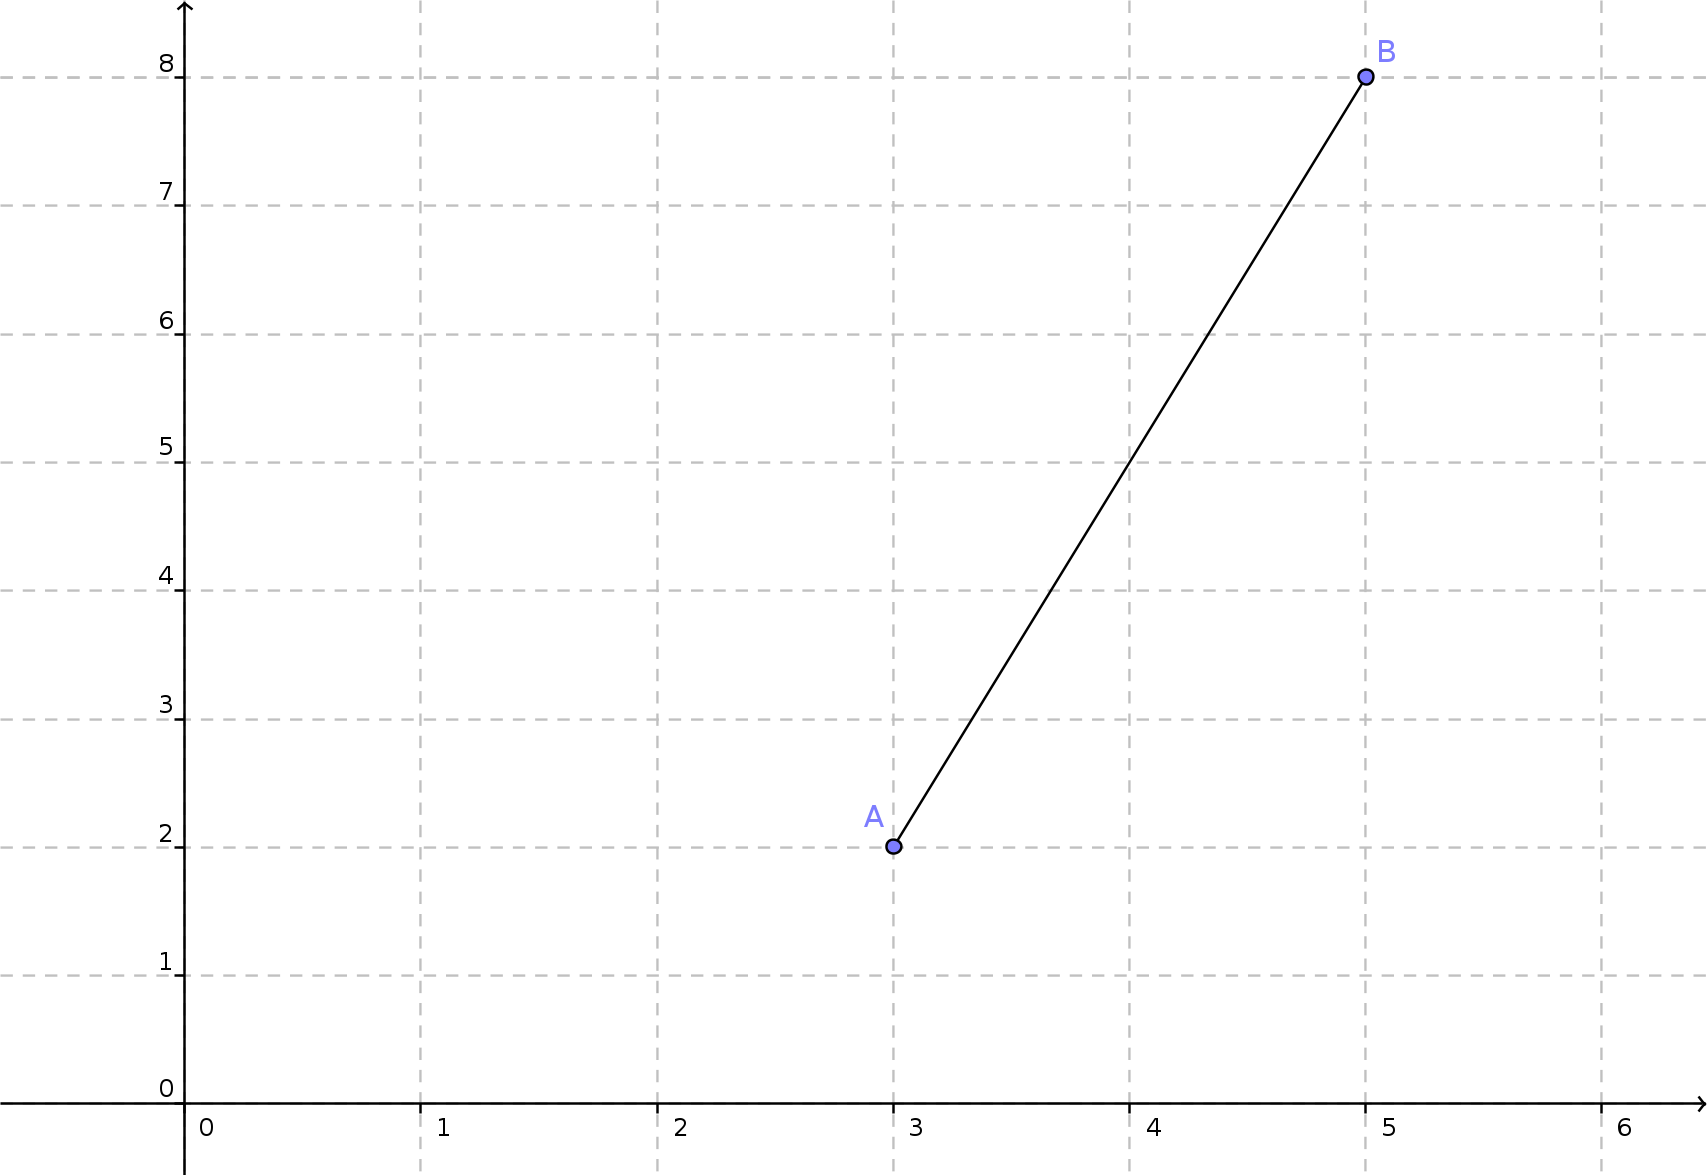
\includegraphics[width=.6\textwidth]{1reta} 
  \caption{Gráfico}
  \label{fig:1reta}
\end{figure}

Resposta: A função da Figura \ref{fig:1reta}:

\begin{displaymath}
  f(x) = 3x-7
\end{displaymath}


\subsubsection{Exemplo 2}

\begin{figure}[h!]
  \centering
  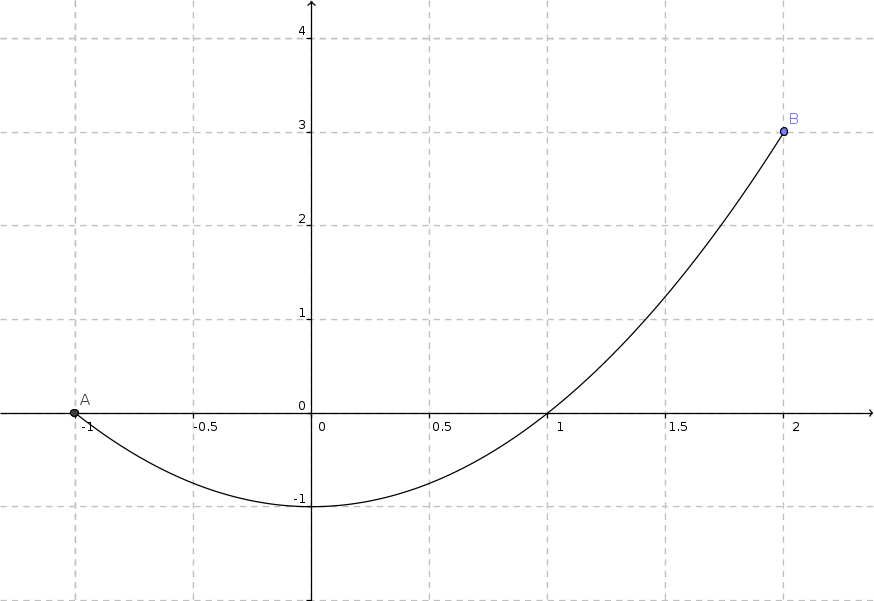
\includegraphics[width=.6\textwidth]{parabola} 
  \caption{Gráfico}
  \label{fig:parabola}
\end{figure}

Resposta: a função da Figura \ref{fig:parabola}:

\begin{displaymath}
  f(x) = x^2-1
\end{displaymath}

está definida para $-1 \le x \le 2$, e sua imagem é $[-1,3]$.

\subsubsection{Exemplo 3}

Podemos também concatenar duas funções

\begin{figure}[h!]
  \centering
  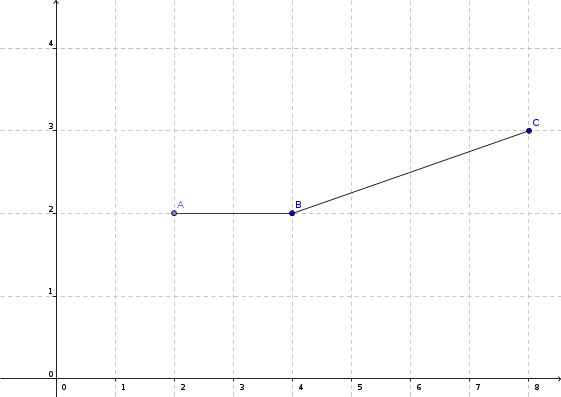
\includegraphics[width=.65\textwidth]{2retas} 
  \caption{Gráfico}
  \label{fig:2retas}
\end{figure}

Resposta: a função da Figura \ref{fig:2retas}:

\begin{displaymath}
  f(x) =   \left\{\begin{tabular}[h]{rc}
                    $2$, & $2 \le x \le 4$\\
                    $\frac{x}{4}+1$, & $x>4$\\
                  \end{tabular}\right.
                \end{displaymath}

está definida para $-1 \le x \le 2$, e sua imagem é $[-1,3]$.

\subsubsection{Exemplo 4}

Para uma concatenação de mais funções, podemos colar duas retas em uma parábola:

\begin{figure}[h!]
  \centering
  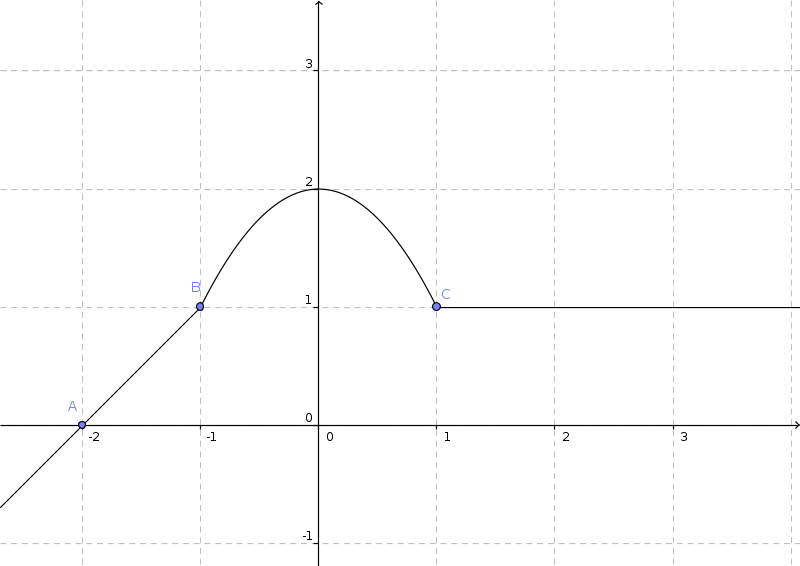
\includegraphics[width=.65\textwidth]{2retas+parabola}
  \caption{Gráfico}
  \label{fig:2retas+parabola}
\end{figure}

Função da Figura \ref{fig:2retas+parabola}:

\begin{displaymath}
  f(x) =
  \left\{\begin{tabular}[h]{rc}
           $x+2$, & $x < -1$ \\
           $-x^2+2$, & $-1 \le x \le 1$ \\
           $1$, & $x > 1$\\ 
  \end{tabular}\right.
\end{displaymath}

Resposta: o domínio é $\mathbb{R}$, e a imagem é $[-\infty, 2]$.

\subsection{Noção de Limite}

\subsubsection{Exemplo 1}

\begin{itemize}
\item Juntar os alunos em duplas;
\item Pegar as calculadoras;
\item Lembrar que na prova {\bf não} será permitida a calculadora
\item Calcular os valores de $f(x)$ para os valores de $x$ abaixo, e preencher a tabela.
\item Caso falte tempo, fazer somente esse na calculadora, e entregar os valores para oos dois últimos exemplos.
\end{itemize}

``Para que valor a função $f(x)$ se aproxima, quando $x$ se aproxima de 1?''

\begin{displaymath}
  f(x) = 2x+3
\end{displaymath}

\begin{multicols}{2}
\begin{tabular}[h]{r|l}
  $x$ & $f(x)$\\
  \hline
0,95 & 4,90 \\
  \hline
0,96 & 4,92\\
  \hline
0,97 & 4,94\\
  \hline
0,98 & 4,96\\
  \hline
0,99 & 4,98\\
\end{tabular}


\begin{tabular}[h]{r|l}
  $x$ & $f(x)$\\
  \hline
1,010 & 5,020\\
  \hline
1,009 & 5,018\\
  \hline
1,008 & 5,016\\
  \hline
1,007 & 5,014\\
  \hline
1,006 & 5,012\\
\end{tabular}

\end{multicols}

\subsubsection{Exemplo 2}

(Neste exemplo, a calculadora ainda vai encontrar uma boa aproximação do limite).

\begin{displaymath}
  f(x) = \frac{x-2}{x^2 - 4}
\end{displaymath}, definida no intervalo $]-2,2[$.

O que acontece com $f$ quando $x$ se aproxima de 2?

\begin{multicols}{2}
\begin{tabular}[h]{r|l}
  $x$ & $f(x)$\\
  \hline
1,95 & 0,25316\\
  \hline
1,96 & 0,25253\\
  \hline
1,97 & 0,25189\\
  \hline
1,98 & 0,25126\\
\hline
1,99 & 0,25063\\
\end{tabular}


\begin{tabular}[h]{r|l}
  $x$ & $f(x)$\\
  \hline
2,010 & 0,24238\\
  \hline
2,009 & 0,24944\\
  \hline
2,008 & 0,24950\\
  \hline
2,007 & 0,24956\\
  \hline
2,006 & 0,24938\\
\end{tabular}

\end{multicols}

Neste ponto, explicar como proceder algebricamente (produto notável, diferença de dois quadrados).

\subsubsection{Exercício}

\begin{displaymath}
  f(x) = \frac{x^2-25}{x + 5}
\end{displaymath}

$f(x)$, definida no intervalo $]-5,5[$.

Usar álgebra para descobrir o que acontece com $f$ quando $x$ se aproxima de -5?

\subsubsection{Exemplo 3}

Agora os alunos verão {\bf porque} não é permitido calculadora nesta disciplina! Eis um exemplo em que a calculadora ``erra''.


\begin{displaymath}
  f(x) = \frac{\sqrt{x^2+9} -3}{x^2}
\end{displaymath}

$f:\mathbb{R}^* \rightarrow \mathbb{R}$, estudar o comportamento de $f$ para $x$ próximo de 0.

   
\begin{multicols}{2}
  \begin{tabular}[h]{c|l}
$x$ & $f(x)$\\
\hline
  \end{tabular}

  \begin{tabular}[h]{c|l}
$x$ & $f(x)$\\
\hline
0,0001 & 0.16666668\\
\hline
0,00001 & 0.16666668\\
\hline
0,000001 & 0.16653345\\
\hline
0,0000001 & 0.17763568\\
\hline
0,00000001 & 0.00000000\\
  \end{tabular}
\end{multicols}

Quando $x$ está perigosamente próximo de 0, a função parece assumir o valor 0. Será que este é o limite?

Não! O limite é $\frac{1}{6}$!

\begin{displaymath}
  \lim_{x \rightarrow 0} \frac{\sqrt{x^2+9} -3}{x^2} =   \lim_{x \rightarrow 0}\frac{\sqrt{x^2+9} -3}{x^2} \times\frac{(\sqrt{x^2+9} +3)}{(\sqrt{x^2+9} +3)}
\end{displaymath}
\begin{displaymath}
 = \lim_{x \rightarrow 0} \frac{\sqrt{x^2+9}^2 - 3^2}{x^2(\sqrt{x^2+9}+3)}
= \lim_{x \rightarrow 0} \frac{\sqrt{x^2+9}^2 - 3^2}{x^2(\sqrt{x^2+9}+3)}
\end{displaymath}
\begin{displaymath}
  =\lim_{x \rightarrow 0} \frac{x^2+(9 - 9)}{x^2(\sqrt{x^2+9}+3)} = \lim_{x \rightarrow 0} \frac{1}{\sqrt{x^2+9}+3}
\end{displaymath}

\begin{displaymath}
 = \lim_{x \rightarrow 0} \frac{1}{\sqrt{9}+3} = \frac{1}{6}
\end{displaymath}
Não confie cegamente na calculadora!
\end{document}
